\chapter{Analasis}
\label{chap:analisis}
Pada bab ini akan dijelaskan analisis masalah penelitian ini. Analisis meliputi Dataset Pada HTTP Archive, Langkah-Langkah Query Yang Dilakukan, 
\section{Dataset Pada HTTP Archive}
Di dalam HTTP Archive terdapat dataset yang dapat diambil menggunakan teknologi BigQuery, dataset tersebut adalah sebagai berikut:
\begin{enumerate}
	\item almanac\\
	Pada tabel ini tidak terdapat keterangan dan tidak berhubungan dengan skripsi ini.
	\item blink$\_$features\\
	Pada tabel ini tidak terdapat keterangan dan tidak berhubungan dengan skripsi ini.
	\item core$\_$web$\_$vitals\\
	Pada tabel ini tidak terdapat keterangan dan tidak berhubungan dengan skripsi ini.
	\item latest\\
	Pada tabel ini tidak terdapat keterangan dan tidak berhubungan dengan skripsi ini.
	\item lighthouse\\
	Dataset pada lighthouse berisi tabel-tabel dari bulan Juni tahun 2017 sampai dengan sekarang yang terdiri dari website pada mobile. Dataset bulan Agustus tahun 2020 baris pada mobile memiliki 6.290.147 baris \ref{table:ct_lh_mobile} yang dapat dianalisis. Masing-masing terdiri dari URL dan report. \textit{URL (Uniform Resource Locator)} merupakan nama-nama domain dan \textit{report}
	\begin{table}[h!]
		\centering
		\begin{tabular}{|l|l|p{7cm}|}
			\hline
			\textbf{Row} & \textbf{url} & \textbf{report}\\
			\hline
			1 & https://proview.dhl.com/ & \\
			\hline
			2 & http://www.actiruta.com/ & \\
			\hline
		\end{tabular}
		\caption{Lighthouse Data Example}
		\label{table:ct_lh_mobile}
	\end{table}
	
	\item pages\\
	Dataset pada pages berisi tabel-tabel dari bulan Januari tahun 2016 sampai dengan sekarang yang terdiri dari website pada desktop dan mobile. Dataset bulan Agustus tahun 2020 baris pada desktop memiliki 5.593.642 baris \ref{fig:ct_pages_desktop} dan pada mobile memiliki 6.347.640 baris \ref{fig:ct_pages_mobile} yang dapat dianalisis. Masing-masing terdiri dari URL dan payload. \textit{URL (Uniform Resource Locator)} merupakan nama-nama domain dan \textit{payload}
	\begin{figure}[H]
		\centering  
		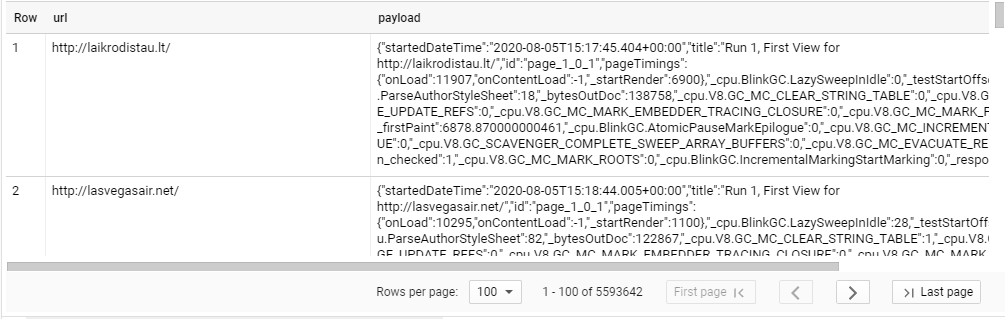
\includegraphics[scale=0.65]{Gambar/2020_08_01_desktop_jumlah_baris_pages.PNG}  
		\caption{Jumlah baris pada tabel pages di desktop} 
		\label{fig:ct_pages_desktop} 
	\end{figure}
	
	\begin{figure}[H]
		\centering  
		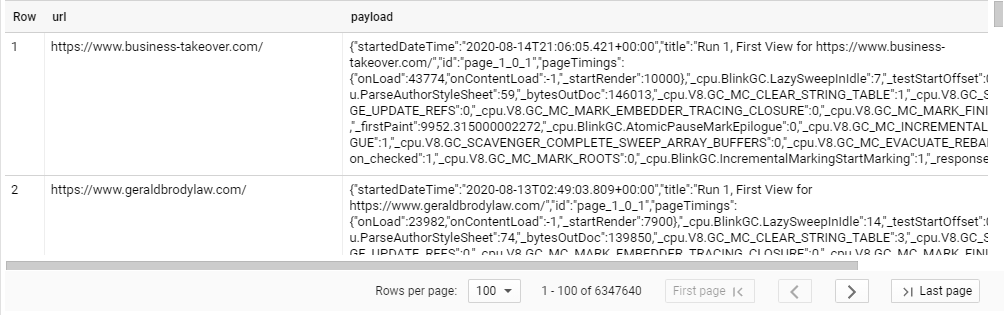
\includegraphics[scale=0.65]{Gambar/2020_08_01_mobile_jumlah_baris_pages.PNG}  
		\caption{Jumlah baris pada tabel pages di mobile} 
		\label{fig:ct_pages_mobile} 
	\end{figure}
	
	\item requests\\
	Dataset pada request berisi tabel-tabel dari bulan Januari tahun 2016 sampai dengan sekarang yang terdiri dari website pada desktop dan mobile. Dataset bulan Agustus tahun 2020 baris pada desktop memiliki 535.841.778 baris dan pada mobile memiliki 579.752.745 baris yang dapat dianalisis. Masing-masing terdiri dari URL dan payload. \textit{URL (Uniform Resource Locator)} merupakan nama-nama domain dan \textit{payload}.
	\item response$\_$bodies\\
	Dataset pada response$\_$bodies berisi tabel-tabel dari bulan Januari tahun 2016 sampai dengan sekarang yang terdiri dari website pada desktop dan mobile. Dataset bulan Agustus tahun 2020 baris pada desktop memiliki 215.621.667 baris dan pada mobile memiliki 270.249.686 baris yang dapat dianalisis. Masing-masing terdiri dari page, URL, body, truncated, dan requestId.
	\item sample$\_$data\\
	Pada tabel ini tidak terdapat keterangan dan tidak berhubungan dengan skripsi ini.
	\item sample$\_$data$\_$2020\\
	Pada tabel ini tidak terdapat keterangan dan tidak berhubungan dengan skripsi ini.
	\item scratchspace\\
	Pada tabel ini tidak terdapat keterangan dan tidak berhubungan dengan skripsi ini.
	\item summary$\_$pages\\
	Dataset pada summary$\_$pages berisi tabel-tabel dari bulan November tahun 2010 sampai dengan sekarang yang terdiri dari website pada desktop dan mobile. Dataset bulan Agustus tahun 2020 baris pada desktop memiliki 5.593.642 baris dan pada mobile memiliki 6.347.919 baris yang dapat dianalisis. Masing-masing terdiri dari pageid, createDate, archive, label, crawlid, wptid, wptrun, url, urlShort, urlhash, cdn, startedDateTime, TTFB, renderStart, onContentLoaded, onLoad, fullyLoad, visualComplete, PageSpeed, SpeedIndex, rank, reqTotal, reqHTML, reqJS, reqCSS, reqImg, reqGif, reqJpg, reqPng, reqFont, reqFlash, reqJson, reqOther, bytesTotal, bytesHTML, bytesJS, bytesCSS, bytesImg, bytesGif, bytesJpg, bytesPng, bytesFont, bytesFlash, bytesJson, bytesOther, bytesHtmlDoc, numDomains, maxDomainReqs, numRedirects, numErrors, numGlibs, numHttps, numCompressed, numDomElements, maxageNull, maxage0, maxage1, maxage30, maxage365, maxageMore, gzipTotal, gzipSavings, $\_$connections, $\_$adult$\_$site, avg$\_$dom$\_$depth, document$\_$height, document$\_$width, localstorage$\_$size, sessionstorage$\_$size, num$\_$iframes, num$\_$scripts, doctype, meta$\_$viewport, reqAudio, reqVideo, reqText, reqXml, reqWebp, reqSvg, bytesAudio, bytesVideo, bytesText, bytesXml, bytesWebp, bytesSvg, num$\_$scripts$\_$async, num$\_$scripts$\_$sync, usertiming.
	\item summary$\_$requests\\
	Dataset pada response$\_$requests berisi tabel-tabel dari bulan November tahun 2010 sampai dengan sekarang yang terdiri dari website pada desktop. Dataset bulan Agustus tahun 2020 baris pada desktop memiliki 215.621.667 baris dan pada mobile memiliki 1.234.599 baris yang dapat dianalisis. Masing-masing terdiri dari requestid, pageid, startedDateTime, time, method, url, urlShort, redirectUrl, firstReq, firstHtml, reqHttpVersion, reqHeaderSize, reqBodySize, reqCookieLen, reqOtherHeader, status, respHttpVersion, respHeaderSize, respBodySize, respSize, respCookieLen, expAge, mimeType, respOtherHeader, req$\_$accept, req$\_$accept$\_$charset, req$\_$accept$\_$encoding, req$\_$accept$\_$language, req$\_$connection, req$\_$host, req$\_$if$\_$modified$\_$since, req$\_$if$\_$none$\_$match, req$\_$referer, req$\_$user$\_$agent, resp$\_$accept$\_$ranges, resp$\_$age, resp$\_$cache$\_$control, resp$\_$connection, resp$\_$content$\_$encoding, resp$\_$content$\_$language, resp$\_$content$\_$length, resp$\_$content$\_$location, resp$\_$content$\_$type, resp$\_$date, resp$\_$etag, resp$\_$expires, resp$\_$keep$\_$alive, resp$\_$last$\_$modified, resp$\_$location, resp$\_$pragma, resp$\_$server, resp$\_$transfer$\_$encoding, resp$\_$vary, resp$\_$via, resp$\_$x$\_$powered$\_$by.
	\item technologies\\
	Dataset pada technologies berisi tabel-tabel dari bulan Januari tahun 2016 sampai dengan sekarang yang terdiri dari website pada desktop dan mobile. Dataset bulan Agustus tahun 2020 baris pada desktop memiliki 61.203.638 baris  dapat dilihat pada gambar \ref{table:ct_tech_desktop} dan pada mobile memiliki 67.452.994 baris \ref{table:ct_tech_mobile} yang dapat dianalisis. Masing-masing terdiri dari 4 kolom yaitu \textit{URL}, \textit{category}, \textit{app}, \textit{info}. Pada kolom \textit{URL (Uniform Resource Locator)} merupakan nama-nama domain, \textit{category} merupakan jenis aplikasi yang digunakan pada website tersebut, \textit{app} merupakan aplikasi yang digunakan website tersebut, \textit{info} merupakan informasi tambahan dari aplikasi. 
	
	\begin{table}[H]
		\centering
		\begin{tabular}{|l|l|p{3cm}|p{3cm}|l|}
			\hline
			\textbf{Row} & \textbf{url} & \textbf{category} & app & info\\
			\hline
			1 & https://www.3-king.com/ & Analytics & Google Analytics & \\
			\hline
			2 & https://www.fleabites.net/ & Miscellaneous & Twitter Emoji (Twemoji) & \\
			\hline
			3 & http://www.elcarnicero.cl/ & Widgets & OWL Carousel & \\
			\hline
			4 & https://thankyou.ws/ & Analytics & Google Analytics & \\
			\hline
			5 & https://rogerwaters.com/ & Reverse proxies & Nginx & \\
			\hline
			6 & http://www.palaciodaslampadas.com.br/ & JavaScript libraries & jQuery & 2.1.1\\
			\hline
			7 & https://copenhagencamping.dk/ & CMS & WordPress & \\
			\hline
			8 & https://eachat.ma/ & Ecommerce & WooCommerce & 4.3.0\\
			\hline
			9 & https://advokat-bondarchuk.ru/ & Blogs & WordPress & \\
			\hline
			10 & https://passport.rsl.ru/ & JavaScript libraries & jQuery & 1.7.1\\
			\hline
		\end{tabular}
		\caption{Technologies Desktop Data Sample}
		\label{table:ct_tech_desktop}
	\end{table}
	
	\begin{table}[H]
		\centering
		\begin{tabular}{|l|l|p{3cm}|p{3cm}|l|}
			\hline
			\textbf{Row} & \textbf{url} & \textbf{category} & app & info\\
			\hline
			1 & http://www.carobd.fr/ & UI frameworks & Bootstrap & 4.1.3\\
			\hline
			2 & http://www.minikabebe.com/ & Font scripts & Font Awesome & \\
			\hline
			3 & https://sibirskisamojedcom.wordpress.com/ & Blogs & WordPress & \\
			\hline
			4 & https://www.peauideale.com/ & Analytics & Google Analytics & \\
			\hline
			5 & https://www.bestcours.com/ & JavaScript libraries & jQuery & 1.11.1\\
			\hline
			6 & https://www.chirurgo-stefanoenrico.it/ & UI frameworks & Bootstrap & \\
			\hline
			7 & https://retrocores.com/ & JavaScript libraries & jQuery & 1.12.4\\
			\hline
			8 & https://pakmule.com/ & Web servers & Apache & \\
			\hline
			9 & https://edilsonalves.com.br/ & JavaScript libraries & jQuery & 1.12.4\\
			\hline
			10 & https://mobilierdasie.com/ & Ecommerce & Google Analytics Enhanced eCommerce & \\
			\hline
		\end{tabular}
		\caption{Technologies Mobile Data Sample}
		\label{table:ct_tech_mobile}
	\end{table}
	
	
	\item urls\\
	Pada tabel ini tidak terdapat keterangan dan tidak berhubungan dengan skripsi ini.
	\item wappalyzer\\
	Pada tabel ini tidak terdapat keterangan dan tidak berhubungan dengan skripsi ini.
\end{enumerate}

\section{Langkah-Langkah Query Yang Dilakukan}
Pada section ini akan dijelaskan tentang langkah-langkah query yang dilakukan dalam memperoleh data dan analisis yang dilakukan. Data yang diambil merupakan dataset dari tabel technologies 2020$\_$08$\_$01:

\subsection{Mencari Aplikasi Yang Digunakan Website}
Setiap website akan dicari aplikasi apa saja yang digunakan dalam pembangunan website tersebut dan versi dari aplikasi yang dipakainya. Berikut adalah query yang digunakan.
\begin{verbatim}
	SELECT url, app, info
	FROM `httparchive.technologies.2020_08_01_*`
	ORDER BY url asc
\end{verbatim}

\subsection{Mengelompokkan Berdasarkan Nama Semua Aplikasi Yang Dipakai}
Pengelompokan aplikasi dapat dilakukan dengan menggunakan query. Berikut adalah query yang digunakan.
\begin{verbatim}
	SELECT app
	FROM `httparchive.technologies.2020_08_01_*`
	GROUP BY app
\end{verbatim}

\subsection{Mencari Data Tentang Versi Aplikasi Yang Masih Didukung}
Sebelum menentukan suatau aplikasi usang atau tidak, kita harus mencari versi dari setiap aplikasi secara manual. Versi setiap aplikasi dapat dilihat di-\textit{official documentation} dari setiap aplikasi. 

\subsection{Melakukan Perbandingan Antara Versi Aplikasi Yang Masih Dipakai Sekarang Dengan Versi Aplikasi Yang Masih Didukung}


\subsection{}

